% Page style for this chapter
	\pagestyle{fancy}
	\lhead{{\sffamily \MakeUppercase{5. Boundary Conditions}}}
	\chead{}
	\rhead{{\sffamily \MakeUppercase\rightmark}}
	\lfoot{}
	\cfoot{{\sffamily \thepage}}
	\rfoot{}
	
\chapter{Boundary Conditions for Monopolar Simulations: A Preliminary
Investigation}
\label{sect:boundary_conditions}

% Textbox
\begin{center}
	\begin{tcolorbox}[title=\boxtitle]
		\begin{itemize}[leftmargin=*,labelindent=2ex,labelsep=1.5ex,itemsep=0pt,parsep=0pt]
			\item How does the prescribed boundary condition affect current flow?
			\item How accurate are the boundary conditions cited in literature?
			\item How do these compare to a whole head simulation?
		\end{itemize}
	\end{tcolorbox}
\end{center}

%% ========================================================= Boundary conditions

\section{Introduction}

As mentioned in Table~\ref{table:model_inputs}, boundary conditions (BCs) are a
key input for volume conduction models (VCMs). If both the source and sink
electrodes are contained within the modelled domain, the BCs are easy to
prescribe. Previous models of bipolar stimulation fall under this
category~\cite{finley1990,frijns1995,hanekom2001,choi2004}. For models of
monopolar (MP) stimulation though, the return electrode lies outside the model
itself, primarily due to restrictions in the field of view during imaging. Since
MP stimulation is by far the most commonly used stimulation mode amongst
contemporary cochlear implant (CI) recipients, it is important to prescribe
boundary conditions that reflect the \invivo{} situation with a reasonable
level of accuracy.

Preliminary tests using the proof of concept model demonstrated that the
restricted scope and extruded geometry of unrolled models are not ideal for
simulating MP current flow~\cite{wong2012}. Here, the medial edge along the base
of the auditory nerve trunk was grounded because earlier studies had identified
this as a likely exit pathway~\cite{vonbekesy1951,girzon1987}. However, imposing
a ground in the nerve trunk itself forces \emph{all} of the injected current to
flow to that point, which is unrealistic because the electrode configuration for
MP stimulation implies that current does not reconverge in the
nerve~\cite{baker1989}. As such, focus was shifted towards the guinea pig and
human models. Looking at the existing literature, it was discovered that a few
different boundary conditions were in use, with little to no consensus amongst
research groups (see Table~\ref{table:existing_bcs}). This raised the need for a
deeper investigation into appropriate BCs.

\begin{table}
	\mathversion{sans}
	\centering
	\sffamily
	\small
	\caption[Monopolar boundary conditions used in existing models]{Monopolar
	boundary conditions used in existing models. For models of the cochlear
	region alone, there appears to be little consensus as to which alternative
	should be used.}
	\label{table:existing_bcs}
	
	\begin{tabularx}{0.58\textwidth}{l X}
		\toprule
		\textbf{Boundary condition \phantom{\hspace{8mm}}}	& \textbf{Key examples} \\
		\midrule
		
		\csvreader[late after line=\\]%
			{Simulations/BCs/literature_bcs.csv}%
			{1=\bc,2=\models}%
 			{\bc & \models}%
		\bottomrule
	\end{tabularx}
	
\end{table}

Ideally, the BCs imposed on a cochlear model would perfectly replicate the
\invivo{} current flow. Unfortunately, it is difficult to measure the volumetric
flow of current in the head during CI stimulation using traditional experimental
techniques. Previous whole head simulations of CI stimulation used crude
geometries and did not focus on volumetric current flow~\cite{mens1999}. Only
recently (through a parallel project) has there been progress in this area, with
the whole head model of
Tran~\etal~\cite{tran2011,tran2013ciap,tran2015,tran2015ciap} revealing the
monopolar current paths.

The aims of this study were twofold: to examine how the model was affected by
changing the BCs, and to compare the predicted current flow patterns with those
from a whole head simulation. This knowledge would help to eliminate potentially
inappropriate boundary conditions from the large set of existing alternatives.

% Spherical and hemispherical symmetry may be important~\cite{ranck1975}.

\section{Grounding Location and Size Effects}

\textit{This section is based on work that was presented at
CIAP2013~\cite{wong2013ciap,tran2013ciap}. The simulations in
Wong~\etal~\cite{wong2013ciap} were from an early iteration of the guinea pig
model; these were rerun using the finalised model for the study in this
chapter.}

The first part of the investigation focused on how various BCs affected the
physics of the system, in particular, the intracochlear voltage profiles and
current pathways. It was hypothesised that both the location/shape and size of
the imposed BCs could affect the simulation results, but the sensitivity of the
model to these factors was unknown.

\subsection{Method}

Several different BCs were established as test cases for this study. These
included grounding at the following surfaces, as shown in
Figure~\ref{fig:bc_meshes}:

\begin{figure}
    \centering
    
    \begin{subfigure}[t]{0.28\textwidth}
        \centering
        \includegraphics[height=4.8cm]{Simulations/BCs/mesh_nrv}
        \caption{}
        \label{fig:bc_mesh_nrv}
    \end{subfigure}%
    \hfill%
    \begin{subfigure}[t]{0.37\textwidth}
        \centering
        \includegraphics[height=4.8cm]{Simulations/BCs/mesh_box}
        \caption{}
        \label{fig:bc_mesh_box}
    \end{subfigure}%
    \hfill%
    \begin{subfigure}[t]{0.35\textwidth}
        \centering
        \includegraphics[height=4.8cm]{Simulations/BCs/mesh_sph}
        \caption{}
        \label{fig:bc_mesh_sph}
    \end{subfigure}%
    
	\caption[Tested grounding locations]{Tested grounding locations highlighted on
	the mesh. (a) The end of the nerve trunk (surrounding bone not shown). (b) The
	boundary box; the surrounding cube is also visible. (c) The surrounding
	spheres; the highlighted sphere has a radius of 5~mm and is circumscribed by
	the surrounding cube in (b). The larger spheres have radii of 10~mm and 20~mm.}
	\label{fig:bc_meshes}
\end{figure}

\begin{description}
	\item[\textsf{The end of the \emph{nerve trunk}}] The truncated end leading
	toward the brain was used here. This was similar to the Girzon and Whiten
	studies, and the rationale can be traced back to measurements by von
	\bekesy~\cite{vonbekesy1960}.
	\item[\textsf{The \emph{boundary box} surrounding the cochlea}] Represents what
	might be used if the model was reconstructed using the image stack alone.
	\item[\textsf{A \emph{surrounding sphere}}] A new proposal inspired by
	Hanekom's use of a surrounding bone block~\cite{hanekom2001} and insights from
	the Tran whole head model~\cite{tran2013ciap}, which revealed that the voltage
	distribution around the cochlea assumes a mostly convex shape (see
	Figure~\ref{fig:bc_head_iso}). The length of the longest diagonal in the
	boundary box was 8.70~mm, so to ensure that none of the cochlear tissues were
	cut off, a sphere of diameter 10~mm was used. Two larger concentric spheres
	with diameters of 20 and 40~mm were also tested.
	\item[\textsf{A \emph{surrounding cube}}] Similar to that used by
	Rattay and Saba. An edge length of 10~mm was used, such that the surrounding
	cube inscribed the surrounding sphere. This allowed for a more direct
	comparison against the spherical BC.
\end{description}

\begin{figure}
    \centering
    
    \begin{subfigure}[t]{0.4\textwidth}
        \centering
        \includegraphics[height=6cm]{Simulations/BCs/head_prelim_volt_net}
        \caption{}
        \label{fig:bc_head_net}
    \end{subfigure}%
    \begin{subfigure}[t]{0.55\textwidth}
        \centering
        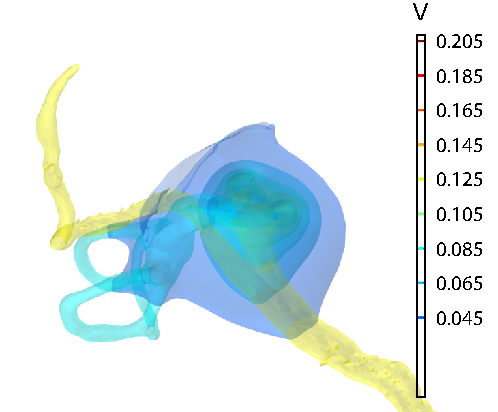
\includegraphics[height=6.2cm]{Simulations/BCs/head_prelim_volt_iso}
        \caption{}
        \label{fig:bc_head_iso}
    \end{subfigure}%
    
	\caption[The shape of the voltage distribution around the cochlea]{The shape of
	the voltage distribution around the cochlea from a whole head simulation. (a)
	Voltage along the surfaces of a surrounding cube; (b) voltage isosurfaces
	around the cochlea take on a mostly convex shape, but is distorted in
	accordance with the modelled tissues.}
	\label{fig:voltage_dist_shape}
\end{figure}

To facilitate the application of these BCs, two volume meshes of the guinea pig
cochlea were created, both of which included all the cochlear tissues and an
electrode array based on the Cochlear Hybrid-L8 (HL8) as described in
\S\ref{sect:gp_mesh_gen}. One mesh included the boundary box and surrounding
cube, whereas the other included the surrounding spheres. This separation was
required to avoid distortions in the mesh where the same sized surrounding
sphere and cube were tangential to each other. The meshes were then imported
into COMSOL for analysis. Only results for current injection at electrode E4 are
presented because the trends were largely independent of the stimulating
electrode.

\subsection{Results}

\subsubsection{Grounding Location}

As shown in Figure~\ref{fig:location_effect_volt}, grounding at different
locations did not seem to have a large effect on the shape of the voltage
profile. This suggests that the voltage drop off is driven by other factors,
likely the geometry and tissue properties. There was, however, a large
discrepancy in the overall magnitude. Grounding the boundary box yielded the
lowest voltages, and the surrounding sphere and cube were slightly higher but
similar to each other. In contrast, the nerve trunk profile was significantly
higher.

\begin{figure}
	\centering
	\includegraphics[height=7cm]{Simulations/BCs/bc_redux_shape}
	\caption[Predicted voltage profile by boundary condition]{Predicted voltage
	profile by boundary condition for the guinea pig model.}
	\label{fig:location_effect_volt}
\end{figure}

The resultant streamline plots (Figure~\ref{fig:location_effect_streams})
revealed that the current pathways were quite different. Grounding the end of
the nerve trunk generated the most distinct flux pattern, with the current
reconverging at the grounded surface and strongly increasing the current density
in the surrounding neural tissue. Using a boundary box constrained the possible
exit pathways, mainly to where the fluid chambers were closest to the centre of
each face of the box. The surrounding sphere and cube were similar except in the
far field, where current was artificially attracted towards the centre of each
face in the cube in a similar manner to the boundary box condition. This
phenomenon is a result of the shorter distance to ground in these regions.

\begin{figure}
    \centering
    
    \begin{subfigure}[t]{0.43\textwidth}
        \centering
        \includegraphics[height=5.5cm]{Simulations/BCs/streamlines-term4-nrv_gnd}
        \caption{Nerve}
        \label{fig:location_effect_streams_nerve}
    \end{subfigure}%
    \begin{subfigure}[t]{0.43\textwidth}
        \centering
        \includegraphics[height=5.5cm]{Simulations/BCs/streamlines-term4-b_box}
        \caption{Boundary box}
        \label{fig:location_effect_streams_box}
    \end{subfigure}%
    \begin{subfigure}[t]{0.09\textwidth}
        \phantom{\hspace{6.4mm}}
    \end{subfigure}\\%
    \vspace{1em}%
    \begin{subfigure}[t]{0.05\textwidth}
        \phantom{\hspace{6.5mm}}
    \end{subfigure}
    \begin{subfigure}[t]{0.43\textwidth}
        \centering
        \includegraphics[height=5.5cm]{Simulations/BCs/streamlines-term4-sph_r5}
        \caption{Sphere (10mm diameter)}
        \label{fig:location_effect_streams_sphere}
    \end{subfigure}%
    \begin{subfigure}[t]{0.43\textwidth}
        \centering
        \includegraphics[height=5.5cm]{Simulations/BCs/streamlines-term4-cube_r5}
        \caption{Cube (10mm edge length)}
        \label{fig:location_effect_streams_cube}
    \end{subfigure}%
    \begin{subfigure}[t]{0.09\textwidth}
        \centering
        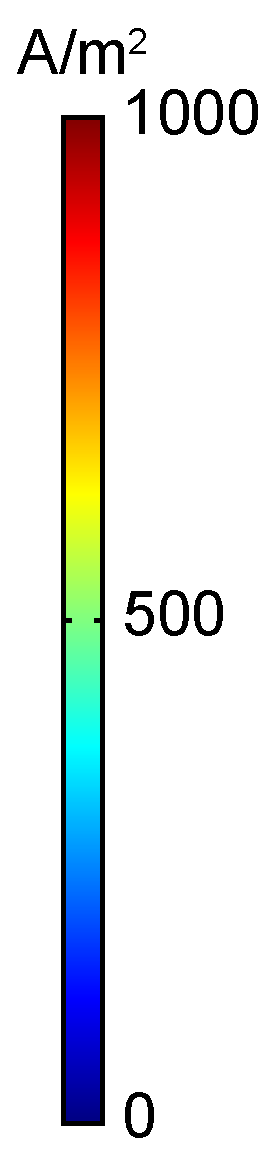
\includegraphics[height=5.5cm]{Validation/cbar_streamlines_short}
    \end{subfigure}%

	\caption[Effect of grounding location on current distribution]{Effect of
	grounding location on current distribution. Scale measured current density in
	the neural tissue.}
	\label{fig:location_effect_streams}
\end{figure}

\subsubsection{Size}

Increasing the size of the surrounding sphere did not have a large impact on
current pathways. Streamlines inside the cochlea barely changed, while those
extending out into the surrounding bone followed an almost perfectly radial
path. Differences were observed in the voltage profiles though, with larger
sizes shifting the curve upwards (Figure~\ref{fig:bc_size_effect}). The marginal
increase appeared to diminish with size, suggesting that a reasonable upper
bound might be proposed by using an infinitely large surrounding sphere.

\begin{figure}
	\centering
	\includegraphics[height=7cm]{Simulations/BCs/bc_redux_size}
	\caption[Effect of size on voltage profile]{Effect of size on voltage profile.
	Increasing the diameter of the surrounding sphere also increased the measured
	voltages, due to the increase in resistance to ground. The marginal change
	appears to diminish with size.}
	\label{fig:bc_size_effect}
\end{figure}

\section{Multiscale Simulation of the Human Head}

The second part of this investigation aimed to compare voltage and current
predictions between standalone models of the cochlea and a multiscale model. It
was hoped that by including reconstructions of both the cochlea and the
surrounding head with realistic return electrodes, a truer sense of the
\invivo{} current distribution would be acquired. Generating an accurate guinea
pig head model was not feasible for this project. Instead, a human multiscale
model was produced in collaboration with a parallel project. This study was
presented at CIAP2015~\cite{tran2015ciap}.

\subsection{Method}

The model of the human inner ear described in \S\ref{sect:human_model} was used
for this study. It was combined with a model of the human head, dubbed HEATHER
(Human ElectroAnatomical Total HEad Reconstruction), which was produced using
anatomical images from female dataset of the Visible Human Project (U.S.
National Library of Medicine, National Institutes of
Health)~\cite{ackerman1997}. Details of the human head reconstruction can be
found in the paper by Tran~\etal~\cite{tran2015}. An image of HEATHER is
provided in Figure~\ref{fig:heather}.

\begin{figure}
	\centering
	\includegraphics[height=9cm]{Simulations/BCs/heather}
	\caption[The HEATHER model]{The HEATHER (Human ElectroAnatomical Total HEad
	Reconstruction) model~\cite{tran2015}. (Copyright \textcopyright{} 2014,
	IEEE.)}
	\label{fig:heather}
\end{figure}

The two models were combined using a process similar to that used previously.
Here, the surfaces extracted from ScanIP for both the inner ear and the head
were imported into ICEM CFD. HEATHER already included a low resolution
reconstruction of the inner ear fluid chambers, serving as a guide for
translating and rotating the reconstruction from this thesis into a near
identical position. The original fluid chambers and facial nerve in HEATHER were
then removed. Computer-aided design (CAD) models of an intracochlear electrode
array with 22 half-banded platinum contacts and a CI implant body were also
included in realistic positions, and a surrounding sphere was added around the
cochlear region to facilitate the comparison of BCs. The radius of the sphere
was 11.5~mm, just sufficient to encompass all of the modelled tissues. Finally,
the entire domain was discretised using the Octree algorithm, and the resultant
NASTRAN mesh was imported into COMSOL for analysis.

In terms of loading, a 106.5~$ \upmu $A current source was applied at electrode
E11, corresponding to a clinical current level of 100 [Cochlear Limited,
internal communication]. Voltage and current patterns were compared for the
following grounding locations:
\begin{itemize}
    \item The end of the nerve trunk;
    \item The surrounding sphere;
    \item The ball electrode (MP1);
    \item The exposed plate on the implant body (MP2).
\end{itemize}

\subsection{Results}

\subsubsection{Model Size and Solution Time}

The combined human model consisted of 10,361,280 tetrahedral elements with an
average element quality of 0.706. Using linear discretisation resulted in a
total of 1,767,281 degrees of freedom (DOFs), which took about 4.5 minutes to
solve.

\subsubsection{Voltage Distribution}

The voltage distribution under MP1, which is typically used in clinical
practice, is shown in Figure~\ref{fig:bc_volt_dist}. A maximum of 0.159~V was
found at the stimulating electrode, corresponding to an impedance of 1.49~k$
\Omega $. Figure~\ref{fig:bc_volt_dist} shows that the electric potential drops
with distance from the stimulating electrode, but it does not fall all the way
to zero near the cochlea itself. This is because the monopolar ground is located
some distance away, just under the scalp.

\begin{figure}
    \centering
    
    \begin{subfigure}[t]{0.4\textwidth}
        \centering
        \includegraphics[width=5cm]{Simulations/BCs/HeadVoltage}
        \caption{}
        \label{fig:bc_voltage_head}
    \end{subfigure}%
    \begin{subfigure}[t]{0.1\textwidth}
        \centering
        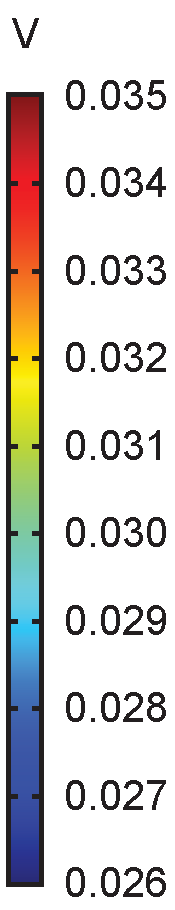
\includegraphics[height=6cm]{Simulations/BCs/legend_head_volt}
    \end{subfigure}%
    \hfill%
    \begin{subfigure}[t]{0.4\textwidth}
        \centering
        \includegraphics[width=5cm]{Simulations/BCs/CochleaVoltage}
        \caption{}
        \label{fig:bc_voltage_coh}
    \end{subfigure}%
    \begin{subfigure}[t]{0.1\textwidth}
        \centering
        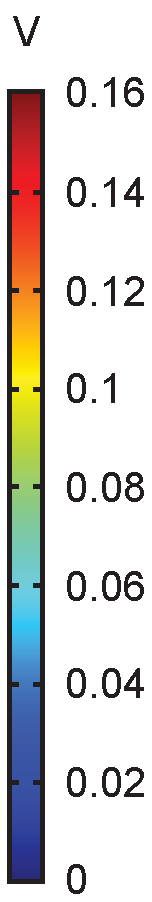
\includegraphics[height=6cm]{Simulations/BCs/legend_coh_volt}
    \end{subfigure}%
    
	\caption[Voltage distribution in the whole head simulation]{Voltage
	distribution in the whole head simulation under MP1 conditions. (a) The entire
	head; (b) the right cochlea only.}
	\label{fig:bc_volt_dist}
\end{figure}

Voltages along the electrode array under the different grounding locations are
plotted in Figure~\ref{fig:heather_coh_voltages}. The trends here were similar
to that shown in Figure~\ref{fig:location_effect_volt} for the guinea pig
model, with little change in the shape of the profile but large shifts in overall
magnitude. MP1 and MP2 produced very similar voltage profiles and represent the
best estimate of the true \invivo{} situation. In comparison to these values,
grounding the nerve trunk overestimated terminal voltages, while grounding the
surrounding sphere underestimated the voltage profile.

\begin{figure}
    \centering
	\includegraphics[height=7cm]{Simulations/BCs/heather_voltages}
	\caption[Predicted \insilico{} terminal voltages by grounding
	location]{Predicted \insilico{} terminal voltages by grounding location for
	the multiscale model.}
	\label{fig:heather_coh_voltages}
\end{figure}

\subsubsection{Current Pathways}

The streamlines also varied between the different cases
(Figure~\ref{fig:bc_streams_man}). There appeared to be three main exit
pathways: (i)~to the spiral ganglion cells next to the stimulating electrode,
then to the nerve trunk, (ii)~to the basal end of the cochlea via the scala
tympani, then to the semicircular canals, and (iii)~through the cochlear walls
and on to the tissues of the head. This is consistent with the findings of
Micco~\cite{micco2006}.

When grounding at the nerve trunk, most of the current travelled through the
cerebrospinal fluid (CSF) surrounding the nerve before converging on the
truncated end surface. Grounding a surrounding sphere produced a weaker sense of
directionality; most of the current still appeared to follow the CSF path, but
there was more flowing via the basal end to the semicircular canals as well as
through the otic capsule towards the cranial cavity and jugular vein. Current
distributions under MP1 and MP2 were even more uniform, and there was very
little difference between these two distant returns.

\begin{figure}
    \centering
    
    \begin{subfigure}[t]{0.4\textwidth}
        \centering
        \includegraphics[width=6cm,trim={0 0 0 8mm},clip]
        {Simulations/BCs/Streamlines_nrv}
        \caption{Grounded at nerve trunk}
        \label{fig:bc_streams_nrv}
    \end{subfigure}%
    \begin{subfigure}[t]{0.4\textwidth}
        \centering
        \includegraphics[width=6cm,trim={0 0 0 8mm},clip]
        {Simulations/BCs/Streamlines_sph}
        \caption{Grounded surrounding sphere}
        \label{fig:bc_streams_sph}
    \end{subfigure}\\%
    \vspace{1em}%
    \begin{subfigure}[t]{0.1\textwidth}
    	\phantom{\hspace{1.55cm}}
    \end{subfigure}%
    \begin{subfigure}[t]{0.4\textwidth}
        \centering
        \includegraphics[width=6cm]{Simulations/BCs/Streamlines_MP1}
        \caption{MP1}
        \label{fig:bc_streams_mp1}
    \end{subfigure}%
    \begin{subfigure}[t]{0.4\textwidth}
        \centering
        \includegraphics[width=6cm]{Simulations/BCs/Streamlines_MP2}
        \caption{MP2}
        \label{fig:bc_streams_mp2}
    \end{subfigure}%
    \begin{subfigure}[t]{0.1\textwidth}
        \centering
        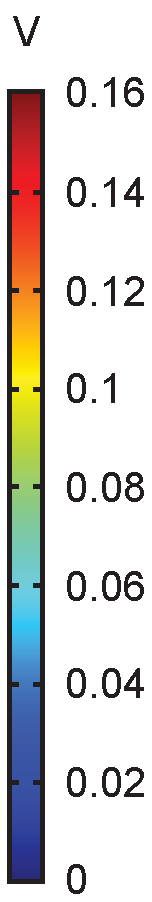
\includegraphics[height=6cm]{Simulations/BCs/legend_coh_volt}
    \end{subfigure}%
    
	\caption[Comparison of current flow patterns]{Comparison of current flow
	patterns for boundary conditions in man. Scale measures the electric potential
	in the neural tissue.}
	\label{fig:bc_streams_man}
\end{figure}

\section{Discussion}

The robustness of the workflow was once again proven by its ability to
successfully create a sophisticated multiscale mesh for finite element (FE)
analysis. The ability to maintain anatomical detail both locally in the cochlear
region as well as throughout the important structures of the head was key to
revealing insights into the expected current flow patterns.

There were several important findings in this study. Perhaps the most pertinent
was that current flows out of the cochlea in all directions, as demonstrated by
the MP1 and MP2 simulations in the multiscale model. There was little difference
between these far-field returns, in line with findings by
Miyamoto~\cite{miyamoto1986}. Current did not flow via the air in the tympanic
cavity however. Considering that the guinea pig cochlea protrudes into the
tympanic bulla (Figure~\ref{fig:guinea_pig_bulla}), it is almost certain that
the current is forced to flow towards the temporal bone in that animal.
Unfortunately, this could not be confirmed in this study due to the lack of a
whole head model of the guinea pig. As such, while guinea pigs might be a good
animal model for studying the cochlea~\cite{miyamoto1986}, simulations of guinea
pig cochleae would likely require the application of BCs that are different from
that for human models. Saba's work indicates that a sense of directionality can
indeed be imposed by using asymmetric boundary conditions where
required~\cite{saba2012}.

The two most traditional BCs---grounding the auditory nerve or the surrounding
bone---exhibited different voltage and current patterns that have hitherto not
been thoroughly examined in the literature. According to these simulations,
neither of them appeared to represent the \invivo{} situation very well.
Grounding the nerve forced current to follow a relatively direct path to the
truncated nerve end, mostly along the highly conductive CSF encasing the
auditory nerve. However, the reconvergence of streamlines seen in
Figures~\ref{fig:location_effect_streams_nerve} and \ref{fig:bc_streams_nrv} is
not realistic because it is only expected to occur at the lone MP return
electrode~\cite{baker1989}, which for MP stimulation is located in the far field
and not in the auditory nerve itself. Even if the cochlear nerve was the
\emph{main} exit pathway, as stipulated by traditional experiments and
lumped-element models, it is incorrect to force \emph{all} of the current
through it, as per Girzon~\cite{girzon1987} and Whiten~\cite{whiten2007}. The
relatively high intracochlear voltages in such implementations
(Figures~\ref{fig:location_effect_volt} and \ref{fig:heather_coh_voltages}) are
a result of the small area of the grounded surface, which increases the overall
resistance.

On a related note, the preferential flow through the CSF jacket around the
auditory nerve suggested that the nerve itself would not be the main exit path,
but the CSF. This makes sense considering the higher conductivity of the CSF and
its connections to other exit pathways through the head~\cite{tran2015}. This
CSF pathway may have been overlooked during early animal experiments because
severing the auditory nerve during extraction of the samples would necessarily
have drained the CSF.

Grounding the bone around the cochlea predicted a more dispersed streamline
pattern than grounding at the nerve. The use of orthogonal bounds (i.e.
along the boundary box or a surrounding cube \`a la
Rattay~\cite{rattay2001model} and Saba~\cite{saba2012}) seemed to be less than
ideal because current was artificially attracted towards the centre of each face
(see Figure~\ref{fig:location_effect_streams}). This was simply because the
surrounding domain was modelled as a homogeneous medium. Since the current
source was closer to the centres than the corners, the lowest resistance path
lay along those trajectories. Using a spherical surrounding surface prevented
these artefacts, while producing similar intracochlear current paths and voltage
predictions. However, the voltages in the scala tympani were still lower than
expected \invivo. Figures~\ref{fig:voltage_dist_shape} and
\ref{fig:bc_volt_dist} suggest that this is because the electric potential
should not be zero at the truncated model boundary; after all, the electric
potential at that location must be some finite amount in order to drive the
current through the remainder of the head tissues to ground.

The voltage predictions were also affected by the size of the surrounding
sphere. As alluded to in the point above, resistance increases with path length,
explaining why the larger shells induced higher voltages. An infinitely large
surrounding sphere per Frijns~\etal~\cite{frijns2000} would treat the system as
a true monopole and induce even higher voltages, but of course the head is not
infinitely large so this may be inappropriate.

Another factor to consider is the resistivity of the surrounding bone domain,
since this would also increase the overall resistance. Previous models of the
human cochlea have assumed a bone to perilymph resistivity ratio of 100:1 in
order to match the predicted potentials~\cite{mens1999,whiten2007,kalkman2014}.
However, changing this value arbitrarily to fit the data is not ideal because
tissue resistivities can be measured accurately~\cite{suesserman1992}.
Setting a value that is too far from the real resistivity can also change the
current paths inside the scalae~\cite{wong2013mb}. For instance, overestimating
bone resistivity would predict an excessive amount of current flowing along the
spiral instead of penetrating the bone. Therefore, it would be better to use
accurately measured values for the tissues in the domain and explain the
remaining voltage difference in terms of the incomplete drop-off arising from
the unmodelled return path through the head to the true MP return.

% Might account for differences in apical vs basal threshold results (see Whiten,
% page 133).

The head is not homogeneous either though. Figure~\ref{fig:voltage_dist_shape}
showed that the tissues immediately surrounding the cochlea distort the electric
field and therefore the resultant current patterns, so ideally this contextual
information should also be incorporated. There are a few ways this might be
done. The first would be to replicate the voltage isosurface from a whole head
model around the standalone cochlear model prior to meshing and apply the
corresponding voltage magnitude over the entire surface in the FE software. This
would be difficult to accomplish due to the complex shape of the isosurface. An
alternative would therefore be to map a non-uniform voltage field onto a
bounding surface whose shape is simple to model, preferably a sphere. The main
challenge in this case would be in getting the locations of the nodes to
match~\cite{wong2013ciap}. For both of these options, the voltage values would
also depend on the magnitude of the stimulus. This could be mitigated by using a
distributed resistance to ground, where the voltage at each node on the
bounding surface is normalised by the normal current density at that point.

Despite these suggestions, it should be noted that the impact on the neural
response was not tested here. It may be insensitive to these changes in the
current distribution because quantities nearer to the current source may be less
affected, and if that were the case then the added complexity of these
alternatives above would not be worth the effort required to implement
them~\cite{bondeson2005}. The model should also be compared to experimental
measurements to validate the predictions. Both of these issues are addressed in
the next chapter.

\section{Conclusions}

Boundary conditions are a key determinant of both intrascalar voltages and
current pathways through the cochlea. It was found that the BCs typically
imposed on cochlear VCMs---grounding either the nerve or the surrounding
bone---induced markedly different voltage profiles and current flow patterns.
A multiscale human model of monopolar CI stimulation was successfully produced
for the first time and demonstrated that neither of these boundary conditions
were robust representations of the expected \invivo{} situation---nerve
grounding appeared to be inappropriate for both guinea pig and human models due
to unrealistic predictions of current flow; grounding a spherical shell around
the cochlea produced more realistic streamlines, but the voltage magnitudes were
lower than expected. Alternative explanations for these differences are explored
in Chapter~\ref{sect:validation}.

% Big difference on overall picture (terminal voltages, streamlines), but minimal
% effect on things closer to the current source (JRC).
